% Drawing 70/07-1 -- folder 70, batch 07, archive page 123 (PDF page 124).
% Transcription: À droite, un polygone régulier (hexagone ou heptagone) dont un sommet et les deux arêtes qui en partent sont repassés en gras, avec un rayon vers le centre ; au-dessous, un cube en perspective où un drapeau (sommet, arête, face) est marqué en gras, avec trois droites étiquetées $\sigma_0$, $\sigma_1$, $\sigma_2$. À côté, la chaîne
% Kind: regular polygon with a bold vertex; cube with a flag. Method 2 (schematic redraw from the facsimile). Status: partial.
% Notes: Right: a regular polygon (drawn as a hexagon) whose top two strokes to the centre are bold (a vertex, its edges and a radius as the transcription reads it: the bold strokes are a V from the top side down to the centre). Below left: a cube in perspective (light strokes) with a flag (vertex, edge, face) in bold and three lines labelled sigma_0, sigma_1, sigma_2 fanning out to the right. The chain of formulas beside it is text.
% Coordinates: 1 unit = 1 mm = 1/100 of the crop width (bbox in page fractions: [0.45, 0.2, 0.95, 0.48]).
% Redrawn by Claude (claude-opus-5-5), issue #73, 2026-11-07; not checked by a human; not compiled (no TeX in the session).
% Rights: reproduces part of the work -- behind RENDER_TRANSCRIPTS, never published by itself.
\documentclass[tikz,border=3pt]{standalone}
\usepackage{amsmath,amssymb}
\usetikzlibrary{patterns,arrows.meta}
\tikzset{pencil/.style={black!45}, struck/.style={black!35}, mark/.style={circle,draw,inner sep=1.3pt}, pt/.style={circle,fill,inner sep=0.9pt}, opt/.style={circle,draw,fill=white,inner sep=1.1pt}}
\begin{document}
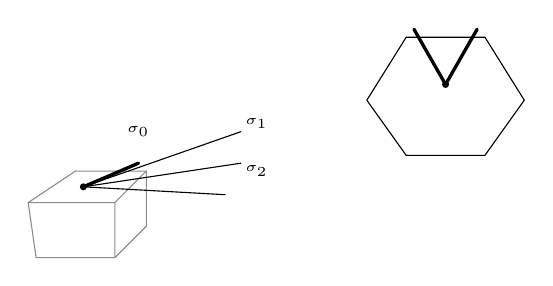
\begin{tikzpicture}[x=1mm,y=1mm,line cap=round,line join=round,font=\scriptsize]
\draw (61,-18) -- (71,-18) -- (76,-26) -- (71,-33) -- (61,-33) -- (56,-26) -- cycle;
\draw[very thick] (62,-17) -- (66,-24);
\draw[very thick] (70,-17) -- (66,-24);
\node[pt] at (66,-24) {};
\draw[pencil] (13,-39) -- (24,-39) -- (24,-46) -- (14,-46) -- cycle;
\draw[pencil] (19,-35) -- (28,-35) -- (28,-42) -- (24,-46);
\draw[pencil] (13,-39) -- (19,-35);
\draw[pencil] (24,-39) -- (28,-35);
\draw[very thick] (20,-37) -- (27,-34);
\node[pt] at (20,-37) {};
\draw (20,-37) -- (40,-30);
\draw (20,-37) -- (40,-34);
\draw (20,-37) -- (38,-38);
\node[inner sep=1pt] at (27,-30) {\tiny $\sigma_0$};
\node[inner sep=1pt] at (42,-29) {\tiny $\sigma_1$};
\node[inner sep=1pt] at (42,-35) {\tiny $\sigma_2$};
\end{tikzpicture}
\end{document}
